\subsection{Zero-Knowledge Proofs and their trust assumptions}

Non-interactive zero-knowledge proofs (NIZKs) are ubiquitous building blocks for achieving both privacy and scalability. Zcash~\cite{zcash} relies heavily on a type of NIZK called a zk-SNARK (zero-knowledge succinct non-interactive argument of knowledge) to prove that a party has sufficient funds to make a payment without revealing anything more about those funds~\cite{SP:BCGGMT14}. On Ethereum, so-called (zk-)rollups enhance scalability by leveraging the succinctness of (zk-)SNARKs, though they may or may not offer the zero-knowledge property.

To achieve such a high level of succinctness, SNARKs rely on a trusted setup to generate a \emph{common reference string (CRS)}. In keeping with the primary innovation of the blockchain, which is the elimination of a trusted third party, practitioners use various approaches to minimize trust in the CRS generation. Zcash uses a multi-party computation ceremony~\cite{zcash-ceremony} with many independent participants to distribute the trust among several parties. Another trust-minimizing approach consists of using SNARKs with universal and updatable CRS~\cite{C:GKMMM18,CCS:MBKM19,EC:CHMMVW20,EPRINT:GabWilCio19}. A universal CRS can be reused across applications, avoiding a new complicated setup ceremony for every use. Updatable CRSs allow any participant in a system to contribute randomness to the CRS at any point, including once the CRS is in production use, to enable a ``one-out-of-many'' trust scenario in which the user must only trust themselves to contribute (and then delete) good randomness to the CRS in order for the whole system to be secure.

An orthogonal concern is maintaining the security of SNARKs when they are composed with other protocols in the complex blockchain ecosystem. Formally, this is modeled by universally composable security via the universal composability (UC) framework~\cite{FOCS:Canetti01}. Unfortunately, most SNARKs in deployment today are not provably UC-secure. Although compilers to transform any SNARK or NIZK into a UC variant exist~\cite{EPRINT:KZMQCP15,EC:GKOPTT23}, these are not compatible with the aforementioned trust-minimizing properties like updatability. A generic compiler which adds UC-security while maintaining updatability would help ensure confidence in both the trusted setup and the operational security of deployed NIZKs.

\renewcommand{\cmark}{\CIRCLE}
\renewcommand{\xmark}{\Circle}
\begin{table}[tbh]
    \centering
    \begin{tabular}{l@{\hspace{1em}} cc cc c}
        \toprule
        & \multicolumn{2}{c}{UC} & \multicolumn{2}{c}{succinctness-preserving}    & \\ \cmidrule(r{3pt}){2-3} \cmidrule(l{3pt}){4-5}
        & SE     & BBE    & in $\lvert C \rvert$ & in $\lvert w \rvert$ & upd. CRS \\
        \midrule
        \COCO~\cite{EPRINT:KZMQCP15}    & \cmark & \cmark & \cmark           & \xmark           & \xmark\\
        DS~\cite{DCC:DerSla19}          & \cmark & \xmark & \cmark           & \cmark           & \xmark\\
        \textsc{Lamassu}~\cite{CCS:AbdRamSla20} & \cmark & \xmark & \cmark           & \cmark           & \cmark\\
        \midrule
        This work \cite{CSF:AGRS24}     & \cmark & \cmark & \cmark           & \xmark           & \cmark\\
        Concurr. work~\cite{EC:GKOPTT23} & \cmark & \cmark & \cmark           & \cmark           & \xmark\\
        \bottomrule
    \end{tabular}
    \caption{Comparison with concurrent and previous work. SE = simulation extractability, BBE = black-box extractability.}\label{tab:comparison}
\end{table}

\subsubsection{Contribution: Circuit-succinct universally composable NIZKs with updatable CRS}

\textit{(Parts of this section are taken/adapted from \cite{CSF:AGRS24}.)}

\usetikzlibrary{fit}
\begin{figure}[tbh]
    \begin{center}
        \begin{tikzpicture}
            \node[draw] (crs_enc) {$\crs_\mathit{enc}$};
            \node[draw] (crs_snark) [right=3em of crs_enc] {$\crs_\mathit{SNARK}$};
            \node[draw] (crs_sig) [right=3em of crs_snark] {$\crs_\mathit{sig}$};
            %
            \node[draw,double] (ucrs_enc) [above=2em of crs_enc] {${\sf u}\crs_\mathit{enc}$};
            \node[draw,double] (ucrs_snark) [above=2em of crs_snark] {${\sf u}\crs_\mathit{SNARK}$};
            \node[draw,double] (ucrs_sig) [above=2em of crs_sig] {${\sf u}\crs_\mathit{sig}$};
            %
            \node[draw] (r_enc) [below=2em of crs_enc] {$\land \mathcal{R}_\mathit{enc}$};
            % pattern=north east lines,fill opacity=0.5
            \node[draw,fill=gray!20] (r_snark) [below=2em of crs_snark] {$\mathcal{R}_\mathcal{L}$};
            \node[draw] (r_sig) [below=2em of crs_sig] {$\lor \mathcal{R}_\mathit{sig}$};
            %
            \node[] (center) [right=1em of r_snark] {};
            \node[] (dspadding) [below=1em of center] {};
            \node[draw,fill=blue,opacity=0.2,inner sep=7pt,fit=(crs_snark) (crs_sig) (r_snark) (r_sig) (dspadding)] (ds) {};
            \node[above] at (ds.south) {DS: non-BB SE};
            %
            \node[] (lamassupadding) [below=2.5em of center] {};
            \node[draw,fill=green,opacity=0.2,inner xsep=15pt,inner ysep=10pt,fit=(ucrs_snark) (ucrs_sig) (r_snark) (r_sig) (lamassupadding)] (lamassu) {};
            \node[above] at (lamassu.south) {\textsc{Lamassu}: upd. non-BB SE};
            %
            % \node[] (topmargin) [above=.5em of crs_snark] {};
            \node[] (cocopadding) [below=3.5em of r_snark] {};
            \node[draw,fill=yellow,opacity=0.2,inner xsep=25pt,inner ysep=13pt,fit=(crs_enc) (crs_sig) (r_enc) (r_sig) (cocopadding)] (coco) {};
            \node[above] at (coco.south) {\COCO: BB SE (UC)};
            %
            \node[] (bblamassupadding) [below=5em of r_snark] {};
            \node[draw,inner xsep=35pt,inner ysep=15pt,fit=(ucrs_enc) (ucrs_sig) (r_enc) (r_sig) (bblamassupadding)] (bblamassu) {};
            \node[above] at (bblamassu.south) {This work: upd. BB SE (UC)};
            %
            \draw[->] (crs_enc)--(ucrs_enc);
            \draw[->] (crs_snark)--(ucrs_snark);
            \draw[->] (crs_sig)--(ucrs_sig);
        \end{tikzpicture}
    % trim=left bottom right top
    % 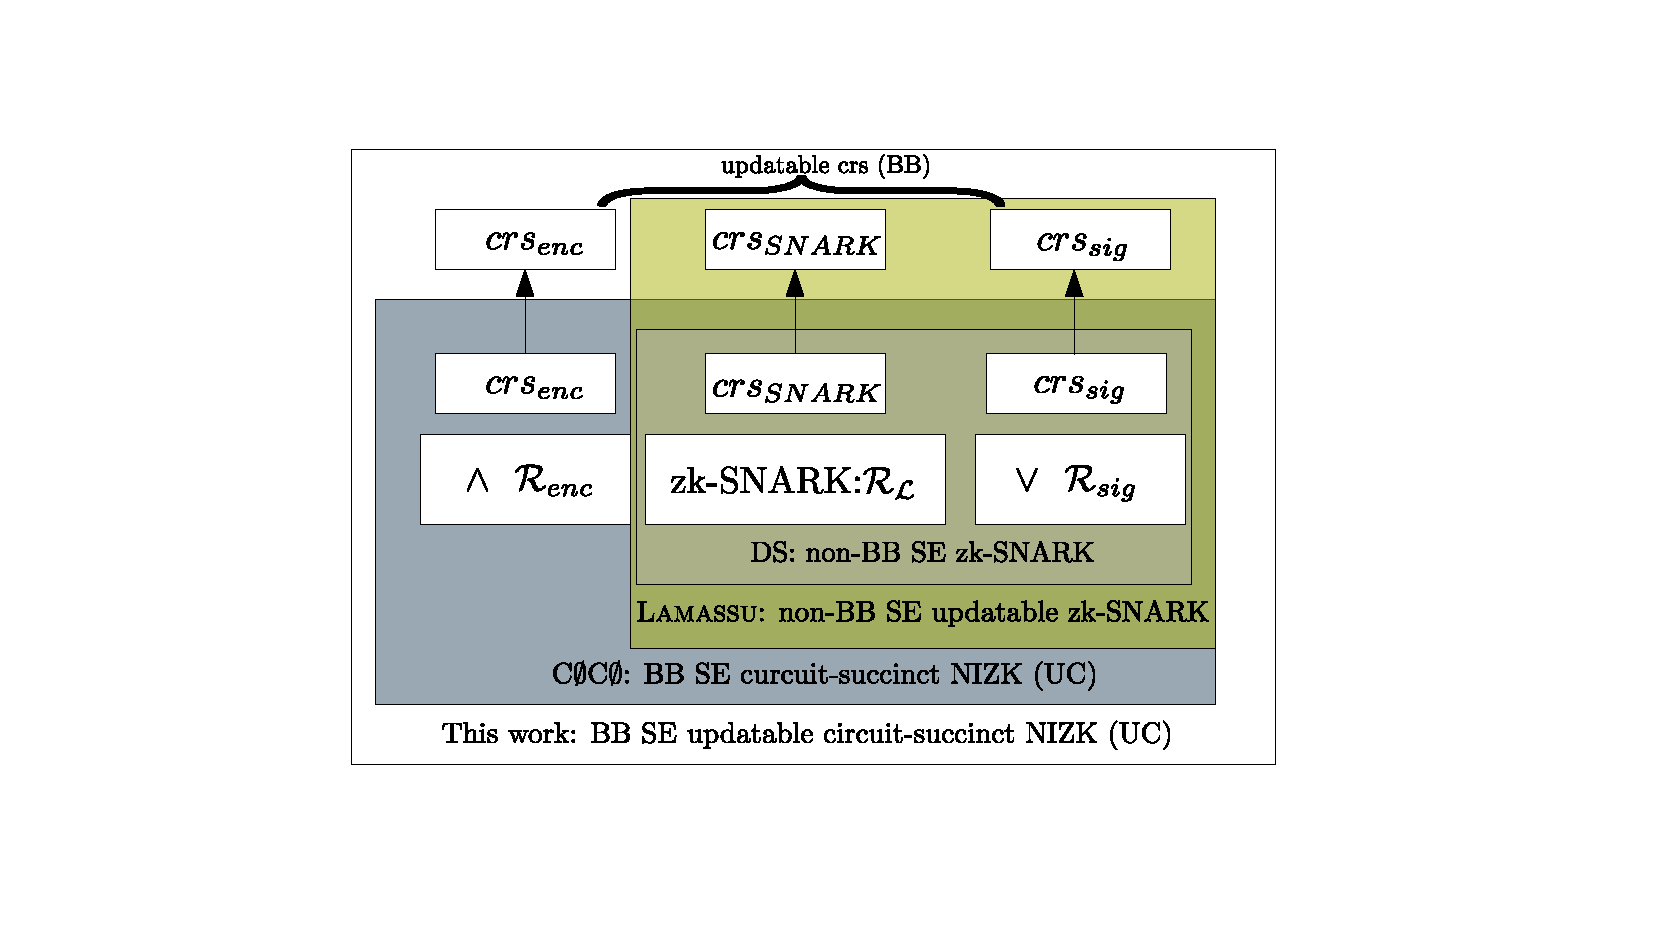
\includegraphics[trim=5.5cm 2.5cm 5cm 2cm, clip, scale =0.5]{overview_new}
    \end{center}
    \caption{Overview of our approach including previous work from Table~\ref{tab:comparison}. ${\sf u}\crs$ denotes an updatable CRS.}
    \label{fig:ucse-overview}
\end{figure}

In \cite{CSF:AGRS24} we show how to build such a compiler by giving the first \emph{fully black-box approach to generically build} circuit-succinct UC-secure NIZKs with updatable CRS from any zk-SNARK, circumventing the aforementioned problems. \textsc{BB-Lamassu} is a framework for black-box (BB) simulation-extractable (SE) (i.e., universally-composable) circuit-succinct NIZKs with updatable CRS. It can be seen as a hybrid of \COCO~\cite{EPRINT:KZMQCP15} and \textsc{Lamassu}~\cite{CCS:AbdRamSla20}, combining the BB extractability of the former with the updatable CRS compatilbility of the latter (see \Cref{tab:comparison}). 
% We follow an approach similar to \COCO\ (grey box) to achieve BB extractability, which as mentioned above requires relaxing the succinctness of SNARKs to that of circuit-succinct NIZKs~\cite{EC:KNYY20} since we need to encrypt the witness in the proof.

\COCO\ (yellow box in \Cref{fig:ucse-overview}) combines two tricks from the literature to achieve BBE and SE. First, to avoid non-black-box extractors that rely on rewinding or knowledge assumptions, they extend the CRS by a public key and include an encryption of the witness in the proof. This also requires extending the original statement to show that the correct witness was encrypted ($\mathcal{R}_{enc}$)~\cite{FOCS:DeSPer92}. Now the extractor can extract the witness by simply decrypting the ciphertext in the CRS. Second, they use the classical OR trick (i.e., an alternate clause $\mathcal{R}_{sig}$, to be used only by the simulator, which checks for a valid signature) to enable unbounded simulation of proofs~\cite{C:DDOPS01}, i.e., SE with a straight-line extractor. Together, these additions augment the underlying scheme with SE and UC-security, but the new ciphertext in the CRS ($\crs_{enc}$) adds a linear overhead of $\sizeof{w}$, so it does not fully preserve succinctness and can only give UC SE \emph{NIZKs}.

\textsc{Lamassu} (green box) revisits the \COCO\ framework, tailoring it to updatable NIZKs and removing the $\sizeof{w}$ overhead. This is achieved by using the non-black-box extractor of the underlying scheme instead of an encryption of the witness, thus preserving succinctness (modulo some small constant overhead). To make unbounded proof simulation compatible with an updatable CRS, \textsc{Lamassu} adapts the simulation technique of \cite{DCC:DerSla19} (blue box), which used the OR trick to combine the underlying SNARK's non-BB extractor with key-homomorphic signatures. To support an updatable CRS, \textsc{Lamassu} swaps the signature for an updatable signature (US). The result is a generic framework for CRS-updatable SE succinct NIZKs, but it sacrifices UC-security due to the non-black-box extractor.

\paragraph{BB-Lamassu.} Our new framework BB-\textsc{Lamassu} (outside box) uses \textsc{Lamassu} as a starting point and adds back in an encryption of the witness ($\mathcal{R}_{enc}$) for BB-extractability. To be compatible with updatability, we instantiate this with a novel public-key encryption (PKE) primitive which we call \emph{extractable key-updatable PKE (EKU-PKE)}, for which we show an efficient construction. 
We still have to overcome the hurdle of providing BB extraction for the US and the public key of the EKU-PKE in the CRS ($crs_{enc}$). In brief, this is done by using an efficient (but not necessarily succinct) BBE NIZK \emph{without a CRS} to prove updates of the CRS elements, i.e., updates of $crs_{SNARK}$, the US public key $crs_{sig}$, and the EKU-PKE public key $crs_{enc}$. 
% \copied{We choose to base these proofs on $\Sigma$-protocols converted to NIZK proofs using either the Fiat-Shamir (FS)~\cite{C:FiaSha86}, Fischlin~\cite{C:Fischlin05} or Unruh~\cite{EC:Unruh15} approach. While this requires that the updates of all components are $\Sigma$-protocol friendly, this holds true for the relations in all known constructions. Interestingly, a byproduct of this approach is that the update proofs for the underlying SNARK CRS become much more efficient to verify (and typically also much smaller). This improvement also carries over to the original \textsc{Lamassu} framework~\cite{CCS:AbdRamSla20} and can be used to improve their CRS update proofs as well.}

\paragraph{UC security proof.}
Since BB-\textsc{Lamassu} is BB SE, it is also UC-secure and should therefore realize the NIZK ideal functionality $\fnizk$ of \cite{AC:Groth06}. However, so far this ignores the updatable CRS aspect. 
To formally confirm this intuition, we introduce a new ideal functionality $\fupcrs$ for the updatable CRS generation and then prove that BB-\textsc{Lamassu} realizes the functionality $\fnizk$ in the $\fupcrs$-hybrid model.
Our analysis is carried out in the local ROM, which can be realized in practice by domain separation in the hash function. We note that the use of an RO arises from a building block (the proof of CRS update) and not from the construction of our compiler. %While we currently consider only the local ROM, we expect that an analysis in the global ROM is possible when relying on Fischlin for the update proofs via the techniques in \cite{TCC:LysRos22}.

\begin{figure}[tb]
    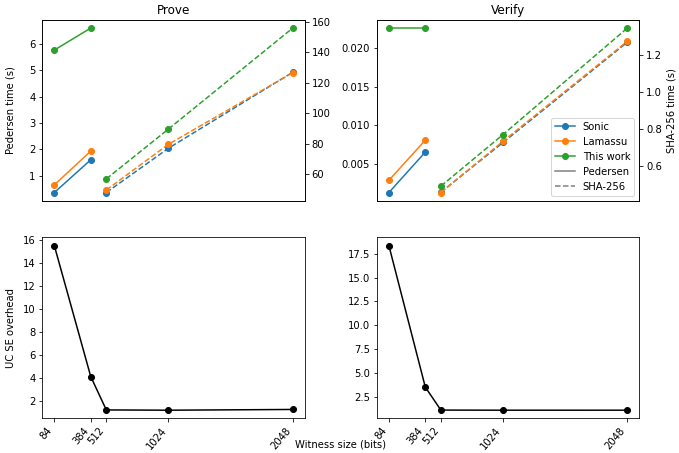
\includegraphics[width=\linewidth]{ucse-benchmarks.png}
    \caption{Runtimes of the Prove and Verify algorithms for Pedersen and SHA-256 preimages using our BB SE succinct NIZK compared to the non-BB SE zk-SNARK obtained via \textsc{Lamassu}~\cite{CCS:AbdRamSla20} and the base non-SE zk-SNARK Sonic~\cite{CCS:MBKM19}. In the lower part we plot the overhead of our transformation to add BB SE, which decreases as the witness size increases.}
    % We do not plot Helped Verify times because they are very small (on the order of hundreds of $\mu$s) and any pattern is overshadowed by noise.
    \label{fig:ucse-eval}
\end{figure}

\paragraph{Performance evaluation.} To demonstrate the applicability of BB-\textsc{Lamassu}, we provide a detailed analysis of the induced overheads. 
For concrete instantiations, we estimate overheads of 32 bytes for the CRS, 170 bytes for the CRS update, and 256 bytes plus the size of the witness for the proof. This is a reduction in both storage and runtime overheads compared to \textsc{Lamassu}~\cite{CCS:AbdRamSla20}.
For witness sizes observed in practical applications such as Zcash, BB-\textsc{Lamassu} adds well below 10,000 additional constraints.

As a concrete example, we apply BB-\textsc{Lamassu} to Sonic~\cite{CCS:MBKM19}, a zk-SNARK with updatable CRS.\footnote{\url{https://github.com/nglaeser/sonic-ucse/}} 
We then experimentally evaluate the overhead introduced by BB-\textsc{Lamassu}. For a SHA-256 preimage, which is interesting for Merkle-tree membership proofs, the prover and verifier overhead, respectively, is $\approx 1.2\times$ and $1.07\times$. Our evaluation shows that as the circuits become larger and more complex, proving and verifying the original circuit dominates the overall performance costs and the overhead added by BB-\textsc{Lamassu} converges to the size of the witness (see \Cref{fig:ucse-eval}).